\subsection{Multiple Objectives in Path-Planning}

% add outline page with current section highlighted.
\begin{frame}{Outline}{ $ \null $ }
	%\tableofcontents[currentsection]
	\tableofcontents[currentsection,currentsubsection]
\end{frame}

\begin{frame}{Pareto Optimal}{Related Work}
%What is Pareto optimal
\begin{columns}
\column{0.4\textwidth}
	\begin{figure}
		\centering
		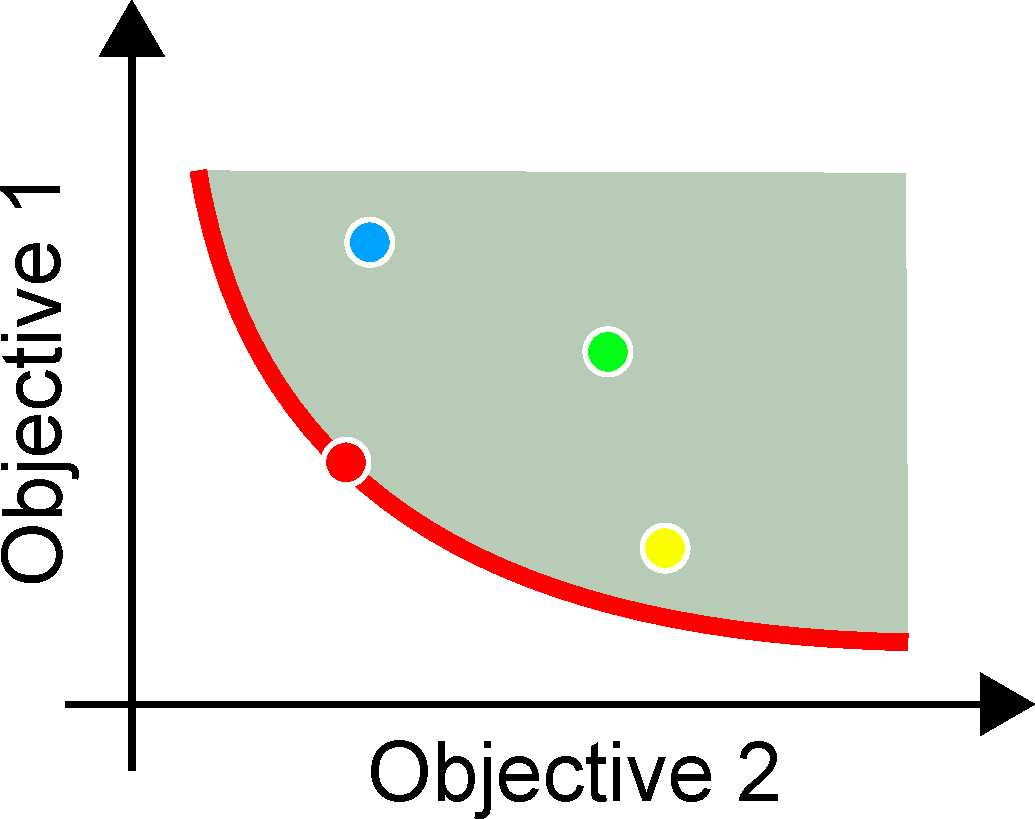
\includegraphics[width=\linewidth]{figure/pareto_optimal}
		%\caption{}
		\label{fig:pareot_optimal}
	\end{figure}
	\begin{center}
	The lower the better
	\end{center}
\column{0.6\textwidth}
\begin{minipage}{\textwidth}
\begin{itemize}
\item $ x_{a} \prec x_{b} $ (dominate)
\begin{itemize}
	\item 
	$ \forall k, f_{k} (x_{a}) \leq f_{k} (x_{b}) $
	\\ $ x_{a} $ is \emph{not worse in all} objectives than $ x_{b} $
	\item 
	$ \exists k, f_{k} (x_{a}) < f_{k} (x_{b}) $
	\\ $ x_{a} $ is \emph{at least better in one} objective than $ x_{b} $
\end{itemize}
\item non-dominant solution $ x^{*} $ \\
\begin{itemize}
	\item there is \emph{no other} solution that can \emph{dominate} $ x^{*} $ \\
	$ \nexists x \in \mathbb{X}, x \prec x^{*} $
\end{itemize}
%\begin{eqnarray*}
%\nexists x \in \mathbb{X}, x \prec x^{*}
%\end{eqnarray*}
\end{itemize}
\end{minipage}
\end{columns}
\end{frame}

\begin{frame}{Finding Pareto Optimal {\em Points} is Hard}{Introduction}
\begin{columns}
\column{0.7\textwidth}
\begin{block}{}
For the point representation
\begin{itemize}
\item \textcolor{diff-path}{constraints}
\item \textcolor{diff-path}{discontinuity}
\item \textcolor{diff-path}{nonconvex}
\item \textcolor{diff-path}{optimality depends on other solutions}
\end{itemize}
\end{block}

\begin{block}{Method}
	\begin{itemize}
		\item NSGA-II
		\item MOEA-D
	\end{itemize}
\end{block}


\column{0.3\textwidth}
	\begin{figure}
		\centering
		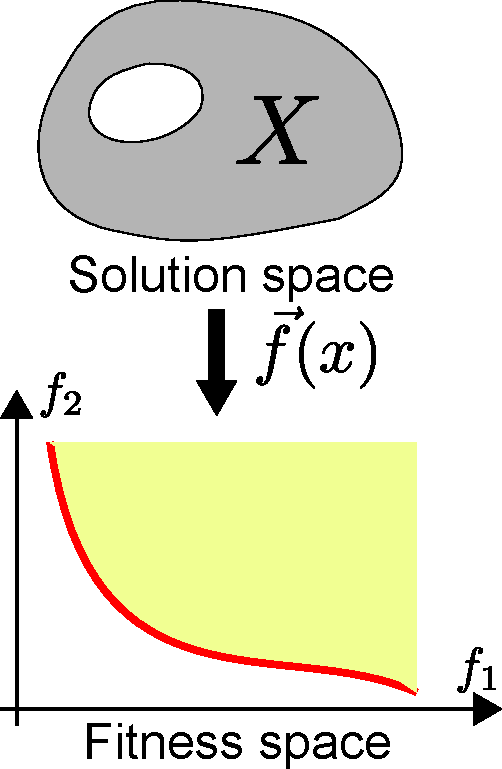
\includegraphics[width=\linewidth]{figure/MOO_point}
		%\caption{}
		\label{fig:point_solution_space}
	\end{figure}
\end{columns}
\end{frame}

%\begin{frame}{Sorting based Approach}{Introduction}

%{\bf NSGA-II}

%\begin{columns}
%\column{0.47\textwidth}
%\begin{figure} 
%	\centering
%	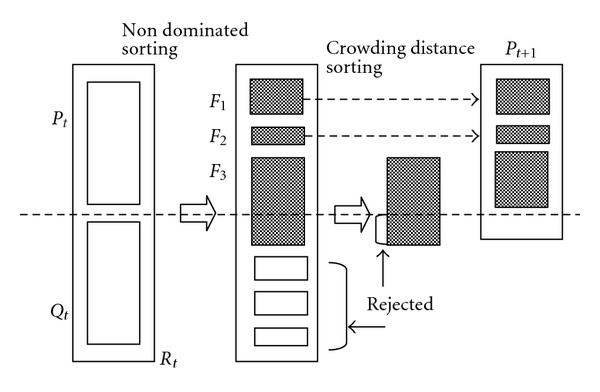
\includegraphics[width=\linewidth]{figure/NSGA_II}
%	\caption{\tiny {\it Yandamuri et al.} ``Multiobjective optimal waste load allocation models for rivers using nondominated sorting genetic algorithm-II.'' Journal of water resources planning and management 2006.}
%\end{figure}

%\column{0.47\textwidth}
%\begin{figure}
%	\centering
%	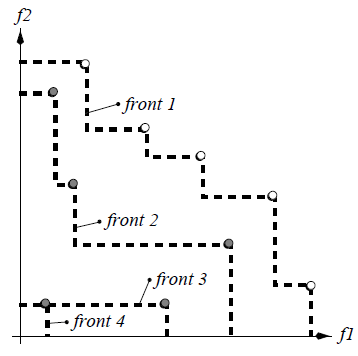
\includegraphics[width=.7\linewidth]{figure/NSGA_II_front}
%	\caption{\tiny {\it Fallahpour et al.} ``Optimization of a LNA Using Genetic Algorithm.'' Electrical and Electronic Engineering 2012.}
%\end{figure}
%\end{columns}

%\end{frame}

%\begin{frame}{Decomposition based Approach}{Introduction}

%{\bf MOEA-D}

%\begin{columns}
%\column{0.47\textwidth}
%\begin{figure}
%	\centering
%	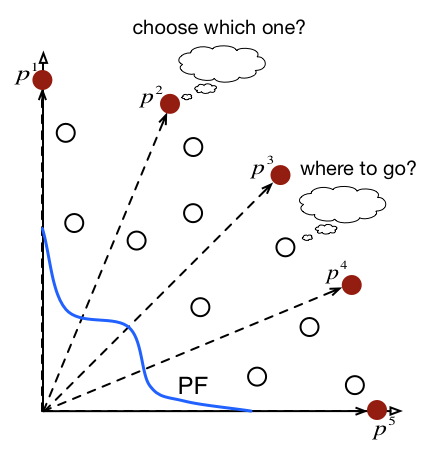
\includegraphics[width=\linewidth]{figure/MOEA-D}
%	\caption{\tiny http://www.cs.cityu.edu.hk/$\sim$51888309/projects.html}
%\end{figure}
%\column{0.47\textwidth}
%\begin{itemize}
%\item Create a set of subproblems for a multi-objective optimization problem
%\item A unique weight vector is assigned to each subproblem
%\item Each subproblem returns a solution 
%\end{itemize}
%\end{columns}

%\end{frame}

\begin{frame}{Finding Pareto Optimal {\em Paths} is Harder}{Introduction}

For the path representation
\begin{itemize}
\item \textcolor{diff-path}{all the properties of the point representation inherited}
\item \textcolor{diff-path}{format inconsistency}
\item \textcolor{diff-path}{fitness accumulation}
%\item high dimension
\end{itemize}

\begin{columns}
\column{0.4\textwidth}
\begin{block}{Format inconsistency}
	\begin{figure}
		\centering
		%\nonumber
		
\includegraphics[width=.6\linewidth]{figure/diff_paths}
		%\caption{Solutions pace}
		%\label{fig:path_solution_space}
	\end{figure}
	\footnotesize{
	It is difficult to map a path into a point in high-dimension space.  
	}
\end{block}
\column{0.5\textwidth}
\begin{block}{Fitness accumulation}
	\begin{figure}
		\centering
		%\nonumber
		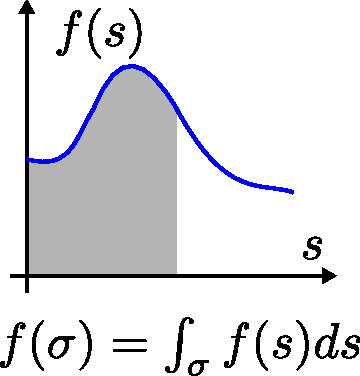
\includegraphics[width=.35\linewidth]{figure/path_integral}
		%\caption{Solutions pace}
		%\label{fig:path_solution_space}
	\end{figure}
	\footnotesize{
	The fitness of a path is the integral of the fitnesses of all visited points.
	}
\end{block}
\end{columns}

\end{frame}

\begin{frame}{Graph-based Approach}{Multi-Objective Path Planning}

{\bf Graph-based Approach}

\begin{columns}
\column{0.6\textwidth}
\begin{itemize}
\item Discretization $ \rightarrow $ graph topology
\item Vector-based cost
\item Multi-objective A$ ^{*}$
\end{itemize}
Drawbacks
\begin{itemize}
\item Low resolution of discretization leads to information loss
\item High resolution of discretization increases the problem size
\end{itemize}
\column{0.4\textwidth}
	\begin{figure}
		\centering
		%\nonumber
		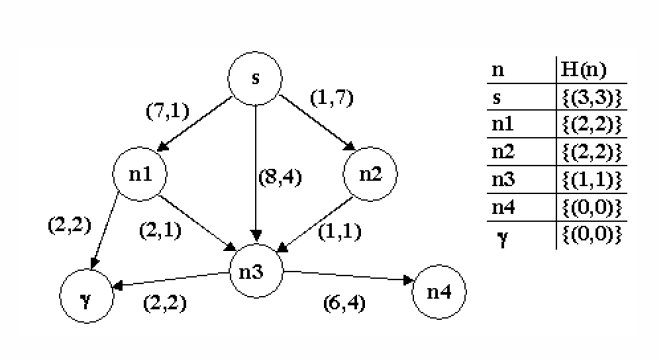
\includegraphics[width=\linewidth]{figure/graph_based_solution.png}
		%\caption{Solutions pace}
		\label{fig:graph_based_solution}
	\end{figure}
\end{columns}

\vfill
\vfill
\vfill

{\tiny {\it Mandow et al.}, ``A new approach to multiobjective A* search''. IJCAI'05}
\clearpage

\end{frame}

\begin{frame}{Point-Equivalence-based Approach}{Multi-Objective Path Planning}

{\bf Point-Equivalence-based Approach}

\begin{columns}
\column{0.6\textwidth}
Model a path as a point in high dimension space
\begin{itemize}
\item Sequence of directions or waypoints
\item Evolutionary algorithm
\begin{itemize}
\item Encode into solution
\end{itemize}
\end{itemize}
Drawbacks
\begin{itemize}
\item obstacles $ \rightarrow $ discontinuity
\item giant search space
\end{itemize}
\column{0.4\textwidth}
	\begin{figure}
		\centering
		%\nonumber
		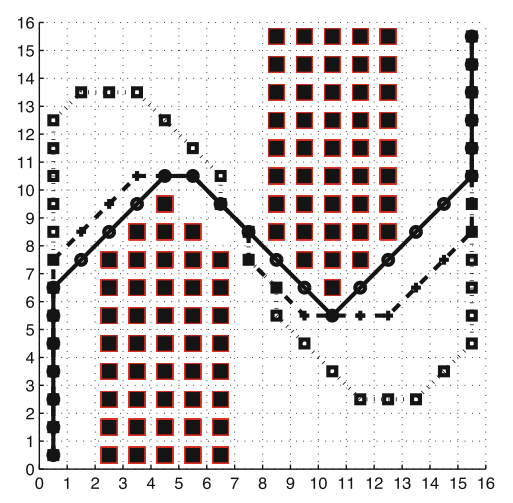
\includegraphics[width=\linewidth]{figure/chain_based_solution.png}
		%\caption{Solutions pace}
		\label{fig:chain_based_solution}
	\end{figure}
\end{columns}

\vfill
\vfill

{\tiny {\it Ahmed et al.}, ``Multi-objective path planning using spline representation''. ROBIO'2011} \\
{\tiny {\it Ahmed et al.}, ``Multi-objective optimal path planning using elitist non-dominated sorting genetic algorithms''. Soft Computing, 2013}
%\clearpage

\end{frame}